\documentclass[xcolor=pdftex,romanian,colorlinks]{beamer}
%\documentclass[xcolor=pdftex,handout,romanian,colorlinks]{beamer}

\usepackage[export]{adjustbox}
\usepackage{../sty/tslides}
\usepackage[all]{xy}
\usepackage{pgfplots}
\usepackage{flowchart}
\usepackage{todonotes}
\usepackage{multicol}  
\usetikzlibrary{arrows,positioning,calc}
\lstset{language=Haskell}
\lstset{escapeinside={(*@}{@*)}}
\PrerenderUnicode{ăĂîÎȘșȚțâÂ}
\usepackage{amsmath}


%\usepackage{xcolor}
%\definecolor{IntensColor}{HTML}{2E86C1}
%\definecolor{StateTransition}{HTML}{D6EAF8}
%\definecolor{MedianLightOrange}{RGB}{216,178,92}
%\definecolor{Orchid}{HTML}{8E44AD}
%\definecolor{True}{HTML}{229954}
%\definecolor{False}{HTML}{CB4335}


\usepackage{proof}
\usepackage{multirow}
\usepackage{alltt}
\usepackage{mathpartir}
\usepackage{ulem}

\newcommand{\structured}[1]{#1}

\definecolor{IntensColor}{HTML}{2E86C1}
\definecolor{StateTransition}{HTML}{D6EAF8}
\definecolor{MedianLightOrange}{RGB}{216,178,92}
\definecolor{Orchid}{HTML}{8E44AD}
\definecolor{True}{HTML}{229954}
\definecolor{False}{HTML}{CB4335}

\newcommand{\cin}[1]{{\color{cobalt} #1}}
\newcommand{\sel}[1]{{\color{Orchid} #1}}

\newcommand{\intens}[1] {{\color{IntensColor} #1}}
\newcommand{\exe}[1] {{\color{True} #1}}

\newcommand{\la}{\lambda}

\setlength{\leftmargini}{0pt}

\newcommand{\app}[2]{#1\, #2}
\newcommand{\abs}[2]{\lambda #1.\,#2}

\newcommand{\type}[2]{{\color{True}#1\hspace{-.05cm}:}\,{\color{Orchid}#2}}

\newcommand{\sub}[3]{#1\langle#2/#3\rangle}
\newcommand{\subt}[3]{#1[#2/#3]}
\newcommand{\equiva}{=_\alpha}

\newcommand{\trueL}{\mathbf{T}}
\newcommand{\falseL}{\mathbf{F}}
\newcommand{\notL}{\mathbf{not}}
\newcommand{\andL}{\mathbf{and}}
\newcommand{\orL}{\mathbf{or}}
\newcommand{\ifL}{\mathbf{if}}
\newcommand{\boolL}{\mathbf{bool}}

\newcommand{\maybeL}{\mathbf{maybe}}
\newcommand{\nothingL}{\mathbf{Nothing}}
\newcommand{\justL}{\mathbf{Just}}
\newcommand{\Maybe}[1]{\mathop{\mathbf{Maybe}}{#1}}

\newcommand{\foldrL}{\mathbf{foldr}}
\newcommand{\nilL}{\mathbf{Nil}}
\newcommand{\consL}{\mathbf{Cons}}
\newcommand{\ListL}[1]{\mathop{\mathbf{List}}{#1}}

\newcommand{\unpairL}{\mathbf{uncons}}
\newcommand{\pairL}{\mathbf{Pair}}
\newcommand{\firstL}{\mathbf{first}}
\newcommand{\secondL}{\mathbf{second}}
\newcommand{\Pair}[2]{\mathop{\mathop{\mathbf{Pair}}{#1}}{#2}}

\newcommand{\succL}{\mathbf{Succ}}
\newcommand{\zeroL}{\mathbf{Zero}}
\newcommand{\iterateL}{\mathbf{iterate}}
\newcommand{\addL}{\mathbf{add}}
\newcommand{\mulL}{\mathbf{mul}}
\newcommand{\expL}{\mathbf{exp}}
\newcommand{\isZero}{\mathbf{isZero}}
\newcommand{\pred}{\mathbf{pred}}
\newcommand{\factL}{\mathbf{fact}}

\newcommand{\BoolT}{\ensuremath{\texttt{Bool}}}
%\newcommand{\BoolT}{\ensuremath{\texttt{Bool}}}
\newcommand{\ifT}[3]{\mathrm{if}\ #1\ \mathrm{then}\ #2\ \mathrm{else}\ #3}

\newcommand{\UnitT}{\ensuremath{\texttt{Unit}}}
\newcommand{\unit}{\mathrm{unit}}

\newcommand{\VoidT}{\ensuremath{\texttt{Void}}}
\newcommand{\void}{\mathrm{void}}


\newcommand{\ProductT}[2]{#1 \times #2}
\newcommand{\PairL}[2]{\langle #1,#2\rangle}
\newcommand{\ProjOne}[1]{fst\ #1}
\newcommand{\ProjTwo}[1]{snd\ #1}

\newcommand{\SumT}[2]{#1 + #2}
\newcommand{\Left}[1]{\mathrm{Left}\ #1}
\newcommand{\Right}[1]{\mathrm{Right}\ #1}
\newcommand{\Case}[3]{\mathrm{case}\ #1\ \mathrm{of}\ #2\ ;\ #3}

%----------------------------------------------

\newcommand{\SSnot}{\terminal{not}}

\newcommand{\Sand}{\terminal{and}}
\newcommand{\Sor}{\terminal{or}}
\newcommand{\Splus}{\terminal{+}}
\newcommand{\Smul}{\terminal{*}}
\newcommand{\Ssucc}{\terminal{S}}
\newcommand{\Spow}{\terminal{pow}}
\newcommand{\Spred}{\terminal{pred}}
\newcommand{\Seq}{\terminal{eq}}
\newcommand{\Sneq}{\terminal{neq}}

\newcommand{\SisZero}{\terminal{isZero}}
\newcommand{\Slte}{\terminal{<=}}
\newcommand{\Sgte}{\terminal{>=}}
\newcommand{\Slt}{\terminal{<}}
\newcommand{\Sgt}{\terminal{>}}
\newcommand{\Spair}{\terminal{pair}}
\newcommand{\Sfst}{\terminal{fst}}
\newcommand{\Ssnd}{\terminal{snd}}
\newcommand{\Sminus}{\terminal{-}}

\newcommand{\Snull}{\terminal{null}}
\newcommand{\Scons}{\terminal{cons}}
%\newcommand{\c sead}{\terminal{head}}
\newcommand{\SisNull}{\terminal{?null}}
\newcommand{\Stail}{\terminal{tail}}
\newcommand{\Ssum}{\terminal{sum}}
\newcommand{\Sfoldr}{\terminal{foldr}}
\newcommand{\Smap}{\terminal{map}}
\newcommand{\Sfilter}{\terminal{filter}}

\newcommand{\const}[1]{\triangleright {\color{False} #1}}

\newcommand{\egf}[1]{\stackrel{\cdot}{=}_{#1}}

\newcommand{\Conf}[2]{\ensuremath{\langle #1\ ,\ #2\rangle}}
\newcommand{\plus}[1] {{\color{True} #1}}
\newcommand{\te}[1]{\mbox{\texttt{#1}}}

\newcommand{\vexp}{\ensuremath{\mathbb{E}}}
\newcommand{\bexp}{\ensuremath{\mathbb{B}}}
\newcommand{\cmd}{\ensuremath{\mathbb{C}}}

\definecolor{section-color}{HTML}{23373b} %mDarkTeal
%\AtBeginSection[]{
%  \begin{frame}
%  \vfill
%  \centering
%  \begin{beamercolorbox}[sep=8pt,center,shadow=true,rounded=true]{title}
%    \usebeamerfont{title}\insertsectionhead\par%
%  \end{beamercolorbox}
%  \vfill
%  \end{frame}
%}



\title[FLP]{Fundamentele limbajelor de programare}
\subtitle{C11}
\date{}


\begin{document}
\begin{frame}
  \titlepage
\end{frame}

\setlength{\leftmargini}{12pt}





%=========================================
\section{\color{section-color}Semantica limbajelor de programare} 
%=========================================

%-------------------------------------------------------------
\begin{frame}{Principalele paradigme de programare}
\begin{itemize}
	\item \intens{Imperativă} (\intens{\underline{cum}} calculăm)
	\vspace{.2cm}
	\begin{itemize}
	\item \intens{Procedurală}
		\vspace{.2cm}
	\item \intens{Orientată pe obiecte}
	
	\end{itemize}
	
	\vspace{.2cm}
	\item  \intens{Declarativă} (\intens{\underline{ce}} calculăm)
		\vspace{.2cm}
	\begin{itemize}
	
	\item \intens{Logică}
	\vspace{.2cm}
	\item \intens{Functională}

	\end{itemize}
\end{itemize}

 \vspace{.2cm}
	\begin{block}{Fundamentele paradigmelor de programare}
		\begin{description}
			\item[Imperativă] Execuția unei Mașini Turing
			\item[Logică] Rezoluția în logica clauzelor Horn
			\item[Funcțională] Beta-reducție în Lambda Calcul
		\end{description}
	\end{block}


\end{frame}



%------------------------------------------------------------------------
\begin{frame}{Ce înseamnă semantică formală?}

\intens{Ce definește un limbaj de programare?}
\medskip  
\begin{itemize}
	\item \intens{Sintaxa} -- Simboluri de operație, cuvinte cheie, descriere (formală) a programelor/expresiilor bine formate
	\medskip	 
	\item \intens{Practic} -- Un limbaj e definit de modul cum poate fi folosit 
	\begin{itemize}
		\item Manual de utilizare și exemple de bune practici
		\item Implementare (compilator/interpretor)
		\item Instrumente ajutătoare (analizor de sintaxă, depanator)
	\end{itemize}
	\medskip  
	\item \intens{Semantica} -- Ce înseamnă/care e comportamentul unei instrucțiuni?
	\begin{itemize}
	\item De cele mai multe ori se dă din umeri și se spune că \structure{Practica} e suficientă 
	\item Limbajele mai utilizate sunt \structure{standardizate}
	\end{itemize}

\end{itemize}
\end{frame}

%------------------------------------------------------------------------
\begin{frame}{La ce folosește semantica?}
\begin{itemize}
	\item Să înțelegem un limbaj în profunzime
	\begin{itemize}
		\item Ca programator: pe ce mă pot baza când programez
		\item Ca implementator al limbajului: ce garanții trebuie să ofer
	\end{itemize}
	\medskip  
	\item Ca instrument în proiectarea unui nou limbaj/a unei extensii 
	\begin{itemize}
		\item \^Ințelegerea componentelor și a relațiilor dintre ele
		\item Exprimarea (și motivarea) deciziilor de proiectare 
		\item Demonstrarea unor proprietăți generice ale limbajului 	
	\end{itemize}
	\medskip  
	\item Ca bază pentru demonstrarea corectitudinii programelor
\end{itemize}
\end{frame}

%-------------------------------------------------------------
\begin{frame}{Problema corectitudinii programelor}

\begin{columns}
\begin{column}{.65\textwidth}
\begin{itemize}
	\item Pentru anumite metode de programare (e.g., imperativă, orientată pe obiecte), nu este ușor să stabilim dacă un program este \intens{corect} sau să  înțelegem ce  înseamnă că este corect (e.g,  în raport cu ce?!). 
	\item \intens{Corectitudinea programelor} devine o problemă din ce  în ce mai importantă, nu doar pentru aplicații "safety-critical".
	\item Avem nevoie de metode ce asigură "calitate", capabile să ofere "garanții".
\end{itemize}
\end{column}
\begin{column}{.4\textwidth}
%\begin{center}
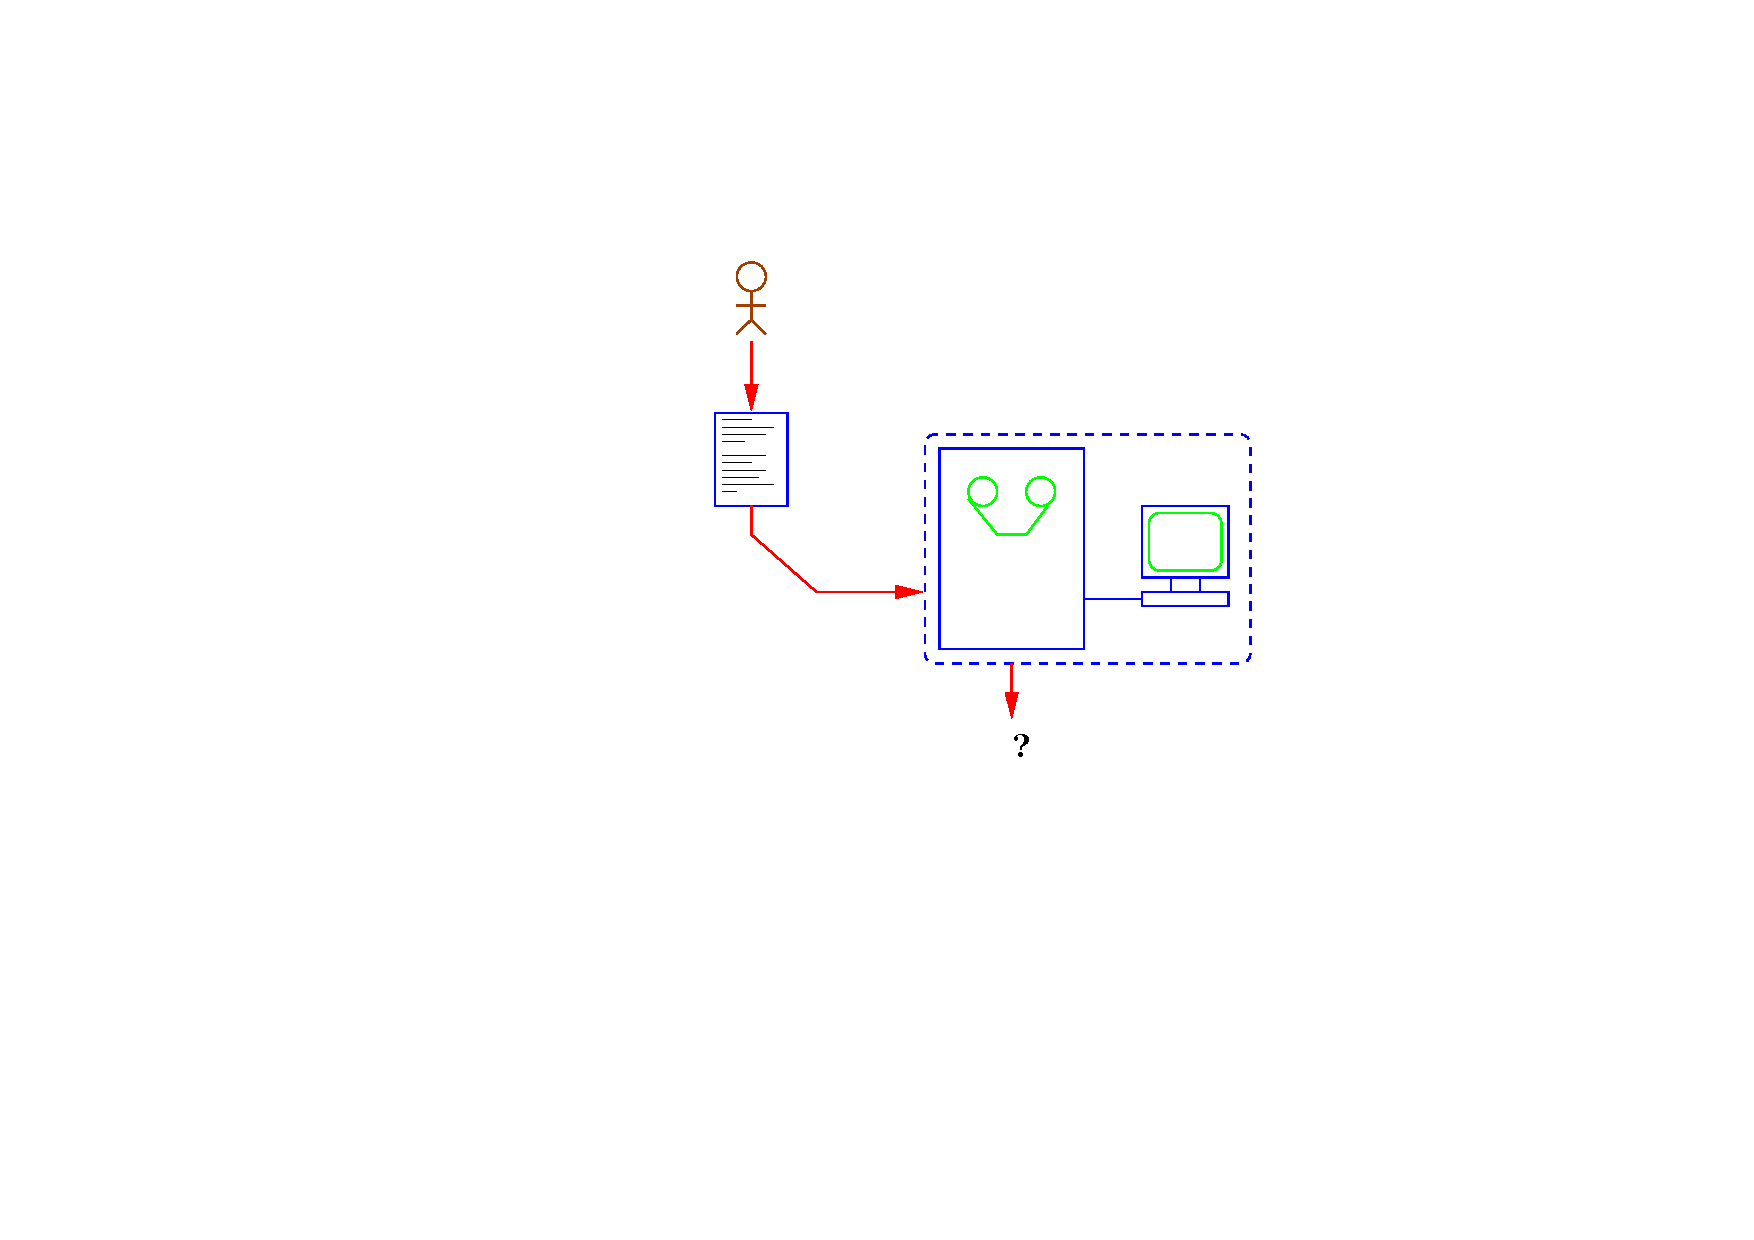
\includegraphics[scale=0.4]{img/imagine1}
%\end{center}
\end{column}
\end{columns}
\end{frame}

%-------------------------------------------------------------
\begin{frame}[fragile]{C}
\begin{columns}
\begin{column}{.5\textwidth}
\begin{verbatim}
#include <iostream> 
using namespace std;
int main() 
{
  int square; 
  for(int i = 1; i <= 5; ++i)
  { 
    square = i * i;
    cout <<  square << endl; 
  }
}
\end{verbatim}
\end{column}
\begin{column}{.5\textwidth}
\begin{itemize}
	\pause \vspace{-.4cm}
	\item \intens{Este corect?} \pause \intens{\^In raport cu ce?}
	\vspace{.2cm}
	\pause
	\item Un \intens{formalism adecvat} trebuie:
	\begin{itemize}
		\item să permită descrierea problemelor (\intens{specificații}), și
		\item să raționeze despre implementarea lor (\intens{corectitudinea programelor}).
	\end{itemize}
\end{itemize}
\end{column}
\end{columns}
\end{frame}

\begin{frame}[fragile]{Care este comportamentul corect?}

\begin{verbatim}
  int main(void) {
    int x = 0;
    return (x = 1) + (x = 2);
  }
\end{verbatim}
\pause
\begin{itemize}
\item GCC4, MSVC: valoarea întoarsă e \alert{4}
\item GCC3, ICC, Clang: valoarea întoarsă e \alert{3}
\end{itemize}
\begin{alertblock}{Conform standardului limbajului C (ISO/IEC 9899:2018)}
  Comportamentul programului este \structure{nedefinit}.
\end{alertblock}
\end{frame}

%------------------------------------------------------------------------
\begin{frame}{Tipuri de semantică}

\vspace{-.1cm}
\begin{itemize}
	\item \intens{Limbaj natural} -- descriere textuală a efectelor
	
	\smallskip  
	\item \intens{Statică} -- un sistem de tipuri care exclude programe eronate

	\smallskip  
	\item \intens{Operațională} -- asocierea unei demonstrații pentru execuție
	\begin{itemize}
		\item $\langle cod, \sigma \rangle  \to  \langle cod', \sigma'\rangle$
		\item modelează execuția unui program pe o mașină abstractă
		\item utilă pentru implementarea de compilatoare și interpretoare
	\end{itemize}

	\smallskip  
	\item \intens{Axiomatică} -- aproximarea logică a efectelor unei instrucțiuni 
	\begin{itemize}
		 \item $\vdash \{\varphi\} cod \{\psi\}$
		\item modelează comportamentul un program prin formulele logice pe care le satisface
		\item utilă pentru demonstrarea corectitudinii
	\end{itemize}
	
	\smallskip  
	\item \intens{Denotațională} -- asocierea unui obiect matematic (denotație)	
	\begin{itemize}
		\item $\llbracket cod \rrbracket$
		\item modelează un program ca obiecte matematice
		\item utilă pentru fundamente matematice
	\end{itemize}	
\end{itemize}
\end{frame}

%------------------------------------------------------------------------
\begin{frame}{Limbajul IMP}

Vom folosi ca exemplu un mic limbaj imperativ IMP care conține:

\begin{itemize}
\item \intens{Expresii}
	\begin{itemize}
		  \item \intens{Aritmetice}: \hspace{.2cm} \texttt{x + 3}
		  \item \intens{Booleene}: \hspace{.2cm} \texttt{x >= 7}
	\end{itemize}
 
\item \intens{Instrucțiuni}
	\begin{itemize}
 		 \item \intens{De atribuire}: \hspace{.2cm} \texttt{x = 5}
		  
 		 \item \intens{Condiționale}: \hspace{.2cm} 
 		 \texttt{if(x >= 7, x = 5, x = 0)}
		  
		  \item \intens{De ciclare}: \hspace{.2cm}
		   \texttt{while(x >= 7, x = x - 1)}
		  \end{itemize}
		   
		  \item \intens{Compunerea instrucțiunilor}: \hspace{.2cm}
		  \texttt{x=7; while(x>=0, x=x-1)}
		   
		  \item \intens{Blocuri de instrucțiuni}: \hspace{.2cm}
		  \texttt{\{x=7; while(x>=0, x=x-1)\}}
\end{itemize}


\end{frame}

%------------------------------------------------------------------------
\begin{frame}[fragile]{Limbajul IMP}


Un exemplu de program în limbajul IMP

\begin{verbatim}
  { x = 10 ; sum = 0;
    while(0 =< x,
       {sum = sum + x; x = x-1}
    )},
    sum      
\end{verbatim}


\intens{Semantica}: dup\u{a} executia programului, se evalueaz\u{a}  \texttt{sum} 


\end{frame}

%----------------------------------------------
  \begin{frame}{Sintaxa BNF a limbajului IMP}
  \vspace{-.2cm}
  \vspace{-5ex}\begin{syntaxBlock}{\AExp}
  \alert{
  \begin{itemize}
  \item[]\renewcommand{\syntaxKeyword}{}
    \syntax{\Int\Smid\Id}{}
%  \syntaxCont{\terminal{++}(\AExp)}{}
  \syntaxCont{\AExp\terminal{+}\AExp\Smid\AExp\terminal{-}\AExp\Smid\AExp\terminal{*}\AExp}{}
     \item[]\renewcommand{\defSort}{\BExp}
  \syntax{\terminal{true}\Smid\terminal{false}}{}
  \syntaxCont{\AExp\terminal{=<}\AExp\Smid \AExp\terminal{>=}\AExp \Smid \AExp\terminal{==}\AExp}{}
  \syntaxCont{\texttt{not}(\BExp) \Smid \texttt{and}(\BExp \terminal{,}\BExp)\Smid \texttt{or}(\BExp \terminal{,}\BExp)}{}
  
  \item[]\renewcommand{\defSort}{\Block}
  \syntax{\terminal{skip}}{}
  \syntaxCont{\Id\terminal{=}\AExp}{}
  \syntaxCont{\Sif\terminal{(}\BExp\terminal{,}\Block\terminal{,}\Block\terminal{)}}{}
  \syntaxCont{\Swhile\terminal{(}\BExp\terminal{,}\Block\terminal{)}}{}
  \syntaxCont{\terminal{\{}\Block\terminal{\}}\Smid \Block\terminal{;}\Block}{}
  \item[]\renewcommand{\defSort}{\Pgm}
  \syntax{\terminal{\{}\Block\terminal{\}}\terminal{,}\AExp}{}
  \end{itemize}
  }
  \end{syntaxBlock}
  \end{frame}



%=========================================
\section{\color{section-color}Semantica operațională small-step} 
%=========================================

\begin{frame}{Imagine de ansamblu}

\begin{itemize}
	\item \intens{Semantica operațională} descrie cum se execută un program pe o masină abstractă (ideală).
	
	\medskip  
	\item \intens{Semantica operațională \textbf{small-step}}
	\begin{itemize}
		\item  semantica structurală, a pașilor mici
		\item descrie cum o execuție a programului avansează în functie de reduceri succesive.
	\begin{center}
	$\langle cod, \sigma \rangle \to   \langle cod', \sigma' \rangle$
	\end{center}
	\end{itemize}
			
	\medskip  
	\item \intens{Semantica operațională \textbf{big-step}}  
	\begin{itemize}
		\item semantică naturală, într-un pas mare
	\end{itemize}
\end{itemize}
\end{frame}

%------------------------------------------------------------------------
\begin{frame}{Starea execuției}

\begin{itemize}
	\item \intens{Starea execuției} unui program IMP la un moment dat este dată de valorile deținute în acel moment de variabilele declarate în program.
	\medskip
	\item Formal, starea execuției unui program IMP la un moment dat este o \intens{funcție parțială} (cu domeniu finit):
	\begin{center}
	$\sigma : Var \rightharpoonup\SInt$ 
	\end{center}
	\medskip  
	\item \intens{Notatii:}
	\begin{itemize}
		\item Descrierea funcției prin enumerare: $\sigma = n \mapsto 10, sum \mapsto 0$
		\item Funcția vidă $\bottom$, nedefinită pentru nicio variabilă
		\item Obținerea valorii unei variabile: $\sigma(x)$
		\item Suprascrierea valorii unei variabile:

$$\sigma_{x\leftarrow v} (y) = \left\{\begin{array}{r@{\mbox{, dacă }}l}
\sigma	(y) & y \neq x \\
v & y = x
\end{array}
\right.$$
	\end{itemize}
\end{itemize}
\end{frame}


%------------------------------------------------------------------------

  \begin{frame}{Semantica small-step}

  \begin{itemize}
  \item Introdusă de Gordon Plotkin (1981) 
  \smallskip
  \item Denumiri alternative: 
  \begin{itemize}
	\item  \structure{S}emantică \structure{O}perațională \structure{S}tructurală
	\item  semantică prin tranziții
	\item  semantică prin reducere
  \end{itemize}
   \smallskip
  \item Definește cel mai mic pas de execuție ca o relație „de tranziție” între configurații:
  \begin{center}
	$\Conf{cod}{\sigma}  \to  \Conf{cod'}{\sigma'}$
  \end{center}
%  \item Fiecare pas de execuție este concluzia unei demonstrații
 \smallskip  
  \item Execuția se obține ca o succesiune de astfel de tranziții:
  
   \smallskip  
  \begin{tabular}{rcl}
  $\Conf{\alert{ x \terminal{=} 0 \terminal{;}}  x \terminal{=} x \terminal{+} 1 }{\bot}$ &  $ \to $  & $\Conf{x \terminal{=} \alert{x} \terminal{+} 1 }{x \mapsto 0}$ \\  
  &$ \to $& $\Conf{x \terminal{=} \alert{0 \terminal{+} 1} }{x \mapsto 0}$ \\  
  &$ \to $& $\Conf{\alert{x \terminal{=} 1 }}{x \mapsto 0}$ \\   
  &$ \to $& $\Conf{\terminal{\{}\terminal{\}}}{x \mapsto 1}$
  \end{tabular}
    
  \item \intens{Cum definim această relație?} \\  Prin inductie după elementele din sintaxă.
    \end{itemize}
  \end{frame}

%------------------------------------------------------------------------
  \begin{frame}{Redex. Reguli structurale. Axiome}
  \bigskip
  \begin{itemize}
  	\item \intens{Expresie reductibilă (redex)}
	\begin{itemize}
		\item  Fragmentul de sintaxă care va fi procesat la pasul următor
	 \end{itemize}
	\begin{center}
	 $\Sif (0 \terminal{<=} 5 \terminal{+} 7 \terminal{*} \alert<2->{x}\terminal{,} r \terminal{=}1\terminal{,}  r \terminal{=}0)$
	 \end{center}
	 \medskip 

	 \item  <3->{\intens{Reguli structurale} 
	 \begin{itemize}
		\item  Folosesc la identificarea următorului redex
		\item Definite recursiv pe structura termenilor
	 \end{itemize}}
	   \onslide<4->{
 $$\reg{
   \Ss{\Conf{\Sif ({b},{\it bl}_1, {\it bl}_2)}{\sigma}}{\Conf{\Sif ({b'}, {\it bl}_1, {\it bl}_2)}{\sigma}}
  }{
    \Ss{\Conf{b}{\sigma}}{\Conf{b'}{\sigma}}
  }
  {}$$
  }
  	
  	\item <5->{\intens{Axiome}
	\begin{itemize}
		\item Realizează pasul computațional
	 \end{itemize}}
	 \vspace{-.2cm}
	 \onslide<6->{$$\reg{\Ss{\Conf{\Sif (\terminal{true},{\it bl}_1, {\it bl}_2)}{\sigma}}{\Conf{{\it bl}_1}{\sigma}}}{}{}$$}
  \end{itemize}
\end{frame}




  

  
\begin{frame}[fragile]{Semantica expresiilor aritmetice}
  \begin{itemize}
    \item \intens{Semantica unui întreg} este o valoare 
  \begin{itemize}
 	\item  nu poate fi redex, deci nu avem regulă
  \end{itemize}
    \smallskip
     \item \intens{Semantica unei variabile}
  	\item[] $\reg[Id]{\Ss{\Conf{x}{\sigma}}{\Conf{i}{\sigma}}}{}{\sigma(x) = i}$

    \smallskip
  \item \intens{Semantica adunării a două expresii aritmetice}	
  \smallskip
    \item[] $\reg[Add]{\Ss{\Conf{i_1 + i_2}{\sigma}}{\Conf{i}{\sigma}}}{}{i_1 + i_2 = i}$
    \medskip  
  \item[] $\reg{\Ss{\Conf{a_1 + a_2}{\sigma}}{\Conf{a_1' + a_2}{\sigma}}}{\Ss{\Conf{a_1}{\sigma}}{\Conf{a_1'}{\sigma}}}{}$
  
  \vspace{.2cm}
  $\reg{\Ss{\Conf{a_1 + a_2}{\sigma}}{\Conf{a_1 + a_2'}{\sigma}}}{\Ss{\Conf{a_2}{\sigma}}{\Conf{a_2'}{\sigma}}}{}$
  
  \vspace{.2cm}
  Observatie: ordinea de  evaluare a argumentelor este nespecificată.
  \end{itemize}
  

\end{frame}




\begin{frame}[fragile]{Semantica expresiilor booleene}
%  {Expresii Booleene. Constante si operatorul de comparație.}
\vspace*{0.5cm}
 
  \begin{itemize}
 

 \item \intens{Semantica operatorului de comparație}
 
 	\smallskip
    $\reg[Leq-false]{\Ss{\Conf{i_1 \terminal{=<} i_2}{\sigma}}  {\Conf{\terminal{false}}{\sigma}}}{}{i_1 > i_2}$
    
    \smallskip
   $\reg[Leq-true]{\Ss{\Conf{i_1 \terminal{=<} i_2}{\sigma}}   {\Conf{\terminal{true}}{\sigma}}}{}{i_1 \leq i_2}$

\bigskip  

 $\reg{\Ss{\Conf{a_1 \terminal{=<} a_2}{\sigma}}  {\Conf{a_1' \terminal{=<} a_2}{\sigma}}}{\Ss{\Conf{a_1}{\sigma}}  {\Conf{a_1'}{\sigma}}}{}\,\,\reg{\Ss{\Conf{a_1 \terminal{=<} a_2}{\sigma}}  {\Conf{a_1 \terminal{=<} a_2'}{\sigma}}}{\Ss{\Conf{a_2}{\sigma}}  {\Conf{a_2'}{\sigma}}}{}$
 
    \bigskip
  \item \intens{Semantica negației} 
   
  \item[] $\reg[!-false]{\Ss{\Conf{\terminal{not(} \terminal{true)}}{\sigma}}  {\Conf{\terminal{false}}{\sigma}}}{}{}$
    
  \item[] $\reg[!-true]{\Ss{\Conf{\terminal{not(} \terminal{false)}}{\sigma}}  {\Conf{\terminal{true}}{\sigma}}}{}{}$
   \bigskip  
  \item[] $\reg{\Ss{\Conf{\terminal{not}(a)}{\sigma}}  {\Conf{\terminal{not}(a')}{\sigma}}}{\Ss{\Conf{a}{\sigma}}  {\Conf{a'}{\sigma}}}{}$
\end{itemize}
 

\end{frame}

\begin{frame}[fragile]{Semantica expresiilor booleene}
%  {Expresii Booleene. Constante si operatorul de comparație.}
\vspace*{0.5cm}
 
  \begin{itemize}
 

 
    \item \intens{Semantica și-ului} 
   
   \smallskip
    \item[] $\reg[And-false]{\Ss{\Conf{\terminal{and}(\terminal{false}\terminal{,} b_2)}{\sigma}}  {\Conf{\terminal{false}}{\sigma}}}{}{}$
      
    \item[] $\reg[And-true]{\Ss{\Conf{\terminal{and}(\terminal{true}\terminal{,}  b_2)}{\sigma}}  {\Conf{b_2}{\sigma}}}{}{}$
     \bigskip
    \item[] $\reg{\Ss{\Conf{\terminal{and}(b_1 \terminal{,} b_2)}{\sigma}}  {\Conf{\terminal{and}(b_1' \terminal{,} b_2)}{\sigma}}}{\Ss{\Conf{b_1}{\sigma}}  {\Conf{b_1'}{\sigma}}}{}$

\end{itemize}
 

\end{frame}


  \begin{frame}[fragile]{Semantica compunerii și a blocurilor}
%  {Expresii Booleene. Constante si operatorul de comparație.}
\vspace*{0.5cm}
 
 
    \begin{itemize}
  \item \intens{Semantica blocurilor} 
  
  \smallskip 
  $\reg[Block]{\Ss{\Conf{\terminal{\{} s \terminal{\}}}{\sigma}}   {\Conf{ s}{\sigma}}}{}{}$
  
  
      \medskip
   \item \intens{Semantica compunerii secvențiale }
   
   \smallskip
   $\reg[Next-stmt]{\Ss{\Conf{\terminal{skip}\terminal{;} s_2}{\sigma}}  {\Conf{s_2}{\sigma}}}{}{}$
   
   \medskip
  $ \reg{\Ss{\Conf{s_1\terminal{;}\ s_2}{\sigma}}  {\Conf{s_1'\terminal{;}\ s_2}{\sigma'}}}{\Ss{\Conf{s_1}{\sigma}}  {\Conf{s_1'}{\sigma'}}}{}$

    \medskip
  \item \intens{Semantica atribuirii} 
  \smallskip
    \item[] $\reg[Asgn]{\Ss{\Conf{x \terminal{=} i}{\sigma}}  {\Conf{\terminal{skip}}{\sigma'}}}{}{\sigma'=\sigma_{x\leftarrow i} }$
   \medskip
  \item[] $\reg{\Ss{\Conf{x \terminal{=} a}{\sigma}}  {\Conf{x \terminal{=} a'}{\sigma}}}{\Ss{\Conf{a}{\sigma}}  {\Conf{a'}{\sigma}}}{}$
  
\end{itemize}
 

  \end{frame}  


\begin{frame}[fragile]{Semantica lui \texttt{if}}
%  {Expresii Booleene. Constante si operatorul de comparație.}
\vspace*{0.5cm}
 
 
    \begin{itemize}
  \item \intens{Semantica lui \texttt{if}} 
 \item[]
  $\reg[If-true]{\Ss{\Conf{\Sif (\terminal{true},{\it bl}_1, {\it bl}_2)}{\sigma}}  {\Conf{{\it bl}_1}{\sigma}}}{}{}$
   
  \item[]
  $\reg[If-false]{\Ss{\Conf{\Sif (\terminal{false},{\it bl}_1,{\it bl}_2)}{\sigma}}  {\Conf{{\it bl}_2}{\sigma}}}{}{}$
   \medskip   
  \item[]
  $\reg{
   \Ss{\Conf{\Sif ({b},{\it bl}_1, {\it bl}_2)}{\sigma}}  {\Conf{\Sif ({b'}, {\it bl}_1, {\it bl}_2)}{\sigma}}
  }{
    \Ss{\Conf{b}{\sigma}}  {\Conf{b'}{\sigma}}
  }
  {}$
  
\vspace{.4cm}
  \item \intens{Semantica lui \texttt{while}} 
  \vspace{-.4cm}
  \item[] \mbox{$\reg[While]{
   \Ss{\Conf{\Swhile ({b},{\it bl})}{\sigma}}  {\Conf{\Sif({b},  {\it bl}\terminal{;}\Swhile({b},{\it bl}),\terminal{skip})}{\sigma}}
  }{}
  {}$}

\vspace{.4cm}
  \item \intens{Semantica programelor} 
  \vspace{.2cm}
  \item[] $\reg[Pgm]{\Ss{\Conf{(\terminal{skip}, a_1)}{\sigma_1}}  {\Conf{(\terminal{skip}, a_2)}{\sigma_2}}}{\Ss{\Conf{a_1}{\sigma_1}}  {\Conf{a_2}{\sigma_2}}}{}$

\vspace{.2cm}
 \item[] \hspace*{0.6cm}$\reg{\Ss{\Conf{(s_1, a)}{\sigma_1}}  {\Conf{(s_2, a)}{\sigma_2}}}{\Ss{\Conf{s_1}{\sigma_1}}  {\Conf{s_2}{\sigma_2}}}{}$  

  
  
\end{itemize}
 

  \end{frame} 
 
%----Executie pas cu pas

%------------------------------------------------------------------------
  \begin{frame}{Semantica small-step a lui IMP}

\intens{Execuție pas cu pas}

  \hspace*{-2em}$\begin{array}{l}
  \Conf{\alert{i \terminal{=} 3} \terminal{;}\ \Swhile (0 \terminal{<=} i \terminal{,}\terminal{\{} i \terminal{=} i \terminal{+} -4 \terminal{\}})}{\bot}\xrightarrow{\textsc{Asgn}}\\
  \pause
  \Conf{\alert{\terminal{skip} \terminal{;}\ \Swhile (0 \terminal{<=} i \terminal{,}\terminal{\{} i \terminal{=} i \terminal{+} -4 \terminal{\}})}}{i \mapsto 3}\xrightarrow{\textsc{Next-stmt}}\\
  \pause
  \Conf{\alert{\Swhile (0 \terminal{<=} i\terminal{,} \terminal{\{} i \terminal{=} i \terminal{+} -4 \terminal{\}})}}{i \mapsto 3}\xrightarrow{\textsc{While}}\\
  \pause
  \Conf{\Sif (0 \terminal{<=} \alert{i}\terminal{,}
 i \terminal{=} i \terminal{+} -4 \terminal{;} 
   \Swhile (0 \terminal{<=} i, \terminal{\{} i \terminal{=} i \terminal{+} -4\terminal{\}}) \terminal{,} \terminal{skip})}{i \mapsto 3}\xrightarrow{\textsc{Id}}\\
  \pause
   \Conf{\Sif (\alert{0 \terminal{<=} 3}\terminal{,}
 i \terminal{=} i \terminal{+} -4 \terminal{;} 
   \Swhile (0 \terminal{<=} i, \terminal{\{} i \terminal{=} i \terminal{+} -4\terminal{\}}) \terminal{,} \terminal{skip})}{i \mapsto 3} \xrightarrow{\textsc{Leq-true}}\\
  \pause
  \Conf{\alert{\Sif (\terminal{true}\terminal{,}
 i \terminal{=} i \terminal{+} -4 \terminal{;} 
   \Swhile (0 \terminal{<=} i, \terminal{\{} i \terminal{=} i \terminal{+} -4\terminal{\}}) \terminal{,} \terminal{skip})}}{i \mapsto 3}\xrightarrow{\textsc{If-true}}\\
  \pause
   \Conf{
 i \terminal{=} \alert{i} \terminal{+} -4 \terminal{;} 
   \Swhile (0 \terminal{<=} i, \terminal{\{} i \terminal{=} i \terminal{+} -4\terminal{\}})}{i \mapsto 3} \xrightarrow{\textsc{Id}}\\ \cdots
  \end{array}$
  \end{frame}
  
%\begin{frame}{Avantaje și dezavantaje}
%
%\intens{Semantica operațională}
%  \begin{itemize}
%  \item[\plus{+}] Definește precis noțiunea de pas computațional
%  \item[\plus{+}] Semnalează erorile, oprind execuția
%  \item[\plus{+}] Execuția devine ușor de urmărit și depanat
%  \item[\alert{--}] Regulile structurale sunt evidente și deci plictisitor de scris
%  \item[\alert{--}] Nemodular: adăugarea unei trăsături noi poate solicita schimbarea întregii definiții
%  \end{itemize}
%
%\end{frame}


%=========================================
\section{\color{section-color}Semantica axiomatică} 
%=========================================

\begin{frame}{Semantica Axiomatică}{Logica Floyd-Hoare}
\begin{itemize}

\item Dezvoltată de Tony Hoare în 1969 \\(inspirată de rezultatele lui Robert Floyd).

\medskip
\item   Definește triplete (\intens{triplete Hoare}) de forma
 \begin{center}
 \intens{$\{P\}$\texttt{ $\cmd$ }$\{Q\}$} 
 \end{center}
 unde:
  \begin{itemize}
    \item $\cmd$ este o instrucțiune 
    
    \medskip
    \item $P$ (precondiție), $Q$ (postcondiție) sunt aserțiuni logice asupra stării sistemului înaintea, respectiv după execuția lui $\cmd$
    
    \medskip
    \item Limbajul aserțiunilor este un limbaj de ordinul I.
 \medskip
 \end{itemize}
%\item Tripletul  $\intens{\{Pre\}\ S\ \{Post\}}$ este (parțial) {\em corect} dac ă:
%\begin{itemize}
%\item dac ă programul se execut ă dintr-o stare inițial ă care satisface \intens{$Pre$}
%\item și execuția se termin ă
%\item atunci se ajunge într-o stare final ă care satisface \intens{$Post$}.
%\end{itemize}
  \end{itemize}
  
 
  \end{frame}


\begin{frame}{Semantica Axiomatică}{Logica Floyd-Hoare}
\begin{block}{Interpretarea unui triplet Hoare \intens{$\{P\}$\texttt{ $\cmd$ }$\{Q\}$}}
\begin{itemize}
\item dacă programul se execută dintr-o stare inițială care satisface \intens{$P$}
\item și execuția se termină
\item atunci se ajunge într-o stare finală care satisface \intens{$Q$}.
\end{itemize}
\end{block}

\pause  \vspace{.2cm}
\textbf{\color{True} Exemple:}
  \begin{itemize}
  \item $\{\texttt{x} = 1\}\ \mbox{\text{x = x+1}}\ \{\texttt{x} =2\}$ este corect
  \item $\{\texttt{x} = 1\}\ \mbox{\texttt{x = x+1}}\ \{\texttt{x} = 3\}$ {\bf nu} este corect
  \item $\{\top\}\ \mbox{\texttt{if (x <= y) z = x; else z = y;}}\ \{\texttt{z} = min(\te{x},\te{y})\}$ este corect
  \end{itemize}
\end{frame}

\begin{frame}
{Logica Hoare ne ajută să verificăm \intens{corectitudinea} programelor}

\begin{itemize}
  \item Se asociază fiecărei construcții sintactice o regulă de deducție

        care definește recursiv tripletele corecte pentru un limbaj.

  \vfill
  \item Se exprimă o aserțiune de corectitudine a programului ca un tripet Hoare

  \vfill
  \item Se verifică dacă tripletul dat e corect folosind definiția recursivă

\end{itemize}
\end{frame}


%----------------------------------------------------------
\begin{frame}{Sistem de reguli pentru logica Floyd-Hoare}

\begin{block}{Reguli generale pentru logică propozițională}

\vfill
\[\reg[$\to$]{\{P1\}\;\cmd\;\{Q1\}}{P1\to P2\si \{P2\}\;\cmd \;\{Q2\}\si 
Q2\to Q1}{}\]

\vfill
\[\reg[$\vee$]{\{P1\vee P2\}\; \cmd \;\{Q\}}{\{P1\}\;\cmd \;\{Q\}\si\{P2\}\;\cmd\;\{Q\}}{}\]
\vfill
\[\reg[$\wedge$]{\{P\}\; \cmd \;\{Q1\wedge Q2\}}{\{P\}\;\cmd \;\{Q1\}\si\{P\}\;\cmd\;\{Q2\}}{}\]
\end{block}

\end{frame}
%------------------------------------------------------------------------
\begin{frame}{Logica Floyd-Hoare pentru IMP1}
\[\reg[Skip]{\{P\}\; \{\} \;\{P\}}{\hspace*{1cm}}{}\]
\vfill
\[\reg[Seq]{\{P\}\;\cmd_1 ; \cmd_2\;\{R\}}{\{P\}\;\cmd_1 \;\{Q\}\si\{Q\}\;\cmd_2\;\{R\}}{}\]
\vfill
\[\reg[Asign]{\{P[x/e]\}\;x = e\;\{P\}}{\hspace*{1cm}}{}\]
\vfill
\[\reg[If]{\{P\}\Sif (\bexp)\  \cmd_1 \Selse \cmd_2\;\{Q\}}{\{\bexp\wedge P\}\;\cmd_1 \;\{Q\}\si\{\neg \bexp\wedge P\}\;\cmd_2\;\{Q\}}{}\]
\vfill
\[\reg[While]{\{P\}\Swhile(\bexp)\,\cmd\;\{\neg \bexp \wedge P\}}{\{\bexp\wedge P\}\;\cmd \;\{P\}}{}\]
\end{frame}

%------------------------------------------------------------------------
\begin{frame}{Regula pentru atribuire}

\[\reg[Asign]{\{P[x/e]\}\;x = e\;\{P\}}{\hspace*{1cm}}{}\]

\textbf{\color{True} Exemplu:}

$\{\texttt{x}+\te{y} = \te{y}+10\}\ \mbox{\texttt{x = x + y}}\ \{\texttt{x} =\te{y}+10\}$ 

\end{frame}

%------------------------------------------------------------------------
\begin{frame}{Regula pentru condiții}



\[\reg[If]{\{P\}\Sif (\bexp)\  \cmd_1 \Selse \cmd_2\;\{Q\}}{\{\bexp\wedge P\}\;\cmd_1 \;\{Q\}\si\{\neg \bexp\wedge P\}\;\cmd_2\;\{Q\}}{}\]

\textbf{\color{True} Exemplu:}

Pentru a demonstra  $\{\top\}\ \mbox{\texttt{if (x <= y) z = x; else z = y;}}\ \{\texttt{z} = min(\te{x},\te{y})\}$
  
  este suficient să demonstrăm 
  \begin{itemize}
	\item  $\{\te{x}\leq\te{y}\}\ \mbox{\texttt{z = x}}\ \{\texttt{z} = min(\te{x},\te{y})\}$
	\item  $\{\neg (\te{x}\leq\te{y})\}\ \mbox{\texttt{z = y}}\ \{\texttt{z} = min(\te{x},\te{y})\}$
  \end{itemize}



\end{frame}

%------------------------------------------------------------------------
\begin{frame}{Invarianți pentru \texttt{while}}
 Cum demonstrăm    \intens{$\{P\}\ \mbox{\texttt{while(\bexp)\ \cmd}}\ \{Q\}$} ? 
\vfill

Se determină un invariant $I$ și se folosește următoarea regulă:

\[\reg[Inv]{\{P\}\Swhile(\bexp)\,\cmd\;\{Q\}}{P\to I\si \{\bexp\wedge I\}\;\cmd \;\{I\}\si (I\wedge \neg{\bexp})\to Q}{}\]



Invariantul trebuie să satisfacă următoarele proprietăți:
\begin{itemize}
\item să fie adevărat inițial
\item să rămână adevărat după execuția unui ciclu
\item să implice postcondiția la ieșirea din buclă
\end{itemize}

\end{frame}

%%------------------------------------------------------------------------
%\begin{frame}[fragile]{Invarianți pentru \texttt{while}}
%$\{\te{x}=n\,\,\wedge\,\, 0\leq x \,\, \wedge \te{y}=1\}$\\
%\begin{verbatim}
%while (0 < x) {y = y * x;  x = x + -1;}
%\end{verbatim}
%$\{\te{y}=n!\}$
%
%\vfill
%\pause
%\begin{itemize}
%\item Invariantul $I$ este \intens{$\te{y} * x!=n!\,\,\wedge 0\leq x$}
%
%\pause
%
%\item $(\te{x}=n\,\,\wedge\,\, 0\leq x \,\, \wedge \te{y}=1)\to I$
%\item $\{I\wedge (0< x)\} \mbox{\texttt{ {
%  y = y * x; x = x + -1; }}} \{\,I\,\}$
%\item $I \wedge \neg(0 < \te{x})\to (\te{y}=n!)$
%
%\end{itemize}
%
%\end{frame}

%------------------------------------------------------------------------
\begin{frame}[fragile]{Invarianți pentru \texttt{while}}
$\{\te{x}=0\,\,\wedge\,\, 0\leq n \,\, \wedge \te{y}=1\}$\\
\begin{verbatim}
while (x < n) { x = x + 1; y = y * x}
\end{verbatim}
$\{\te{y}=n!\}$

\vfill
\pause
\begin{itemize}
\item Invariantul $I$ este \intens{$\te{y}=x!$}

\pause

\item $(\te{x}=0\,\,\wedge\,\, 0\leq n \,\, \wedge \te{y}=1)\to I$
\item $\{I\wedge (x < n)\} \mbox{\texttt{ {
   x = x + 1; y = y * x}}} \,\,\{\,I\,\}$
\item $I \wedge \neg(\te{x} < n)\to (\te{y}=n!)$

\end{itemize}

\end{frame}


%---------------------------------------------
\begin{frame}
  \vfill
  \centering

\textbf{Pe data viitoare!}

  \vfill
\end{frame}

\end{document}







